\chapter{Il cervello: una storia lunga 500 milioni di anni}

\begin{quotation}
``L'evoluzione è conservatrice: non butta mai via nulla che possa essere riciclato.''\\
---Neil Shubin
\end{quotation}

Se il primo capitolo ci ha mostrato il \textit{cosa} e il \textit{perché} dei nostri bias cognitivi, è ora di esplorare il \textit{quando} e il \textit{come}. Quando, nella lunga storia della vita sulla Terra, sono emersi questi meccanismi mentali che oggi ci fanno controllare ossessivamente lo smartphone? Come si sono stratificati, uno sopra l'altro, fino a creare l'affascinante pasticcio neurologico che chiamiamo mente umana?

Quello che state per leggere è un viaggio attraverso mezzo miliardo di anni di bricolage neurologico, dove ogni tappa evolutiva ha aggiunto nuovi strumenti senza mai rimuovere quelli precedenti. È la storia di come siamo arrivati ad avere, nella stessa scatola cranica, il sistema di allerta di un pesce primitivo, l'aggressività territoriale di un rettile, l'ansia sociale di un mammifero, e la capacità di autoanalisi di un primate. E di come tutti questi sistemi, progettati per epoche completamente diverse, ora tentino di gestire notification push e algoritmi di machine learning.

\section{L'alba della cognizione: il primo interruttore}

\begin{figure}[H]
    \centering
    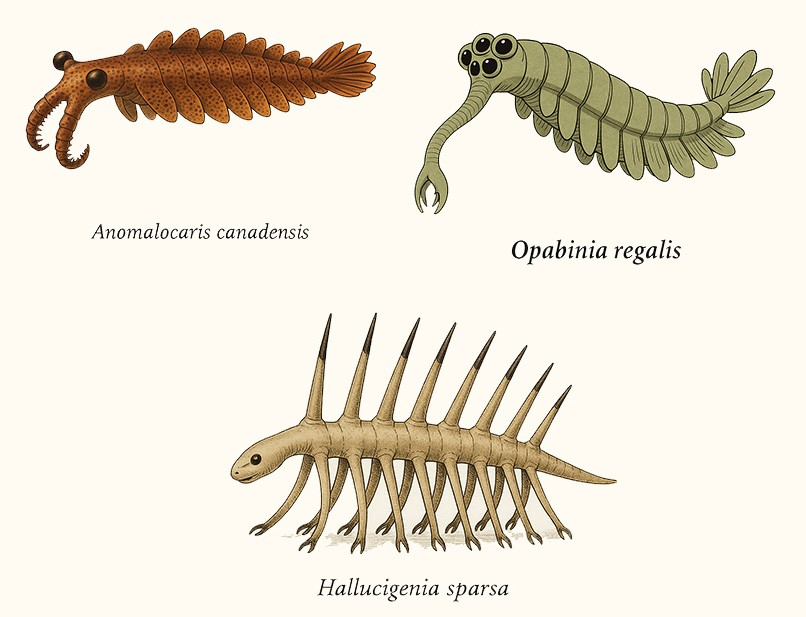
\includegraphics[width=0.5\textwidth]{images/cambriano_alieni.jpg}
    \caption{Le bizzarre creature del Cambriano: una ricostruzione di \textit{Anomalocaris}, \textit{Opabinia} e \textit{Hallucigenia}. Da questi primi esperimenti evolutivi, simili a creature lovecraftiane, sono emersi i primi e più semplici sistemi nervosi.}
    \label{fig:creature_cambriane}
\end{figure}

Immergiamoci nelle acque torbide del Cambriano, 550 milioni di anni fa. Qui nuotano creature che sembrano uscite da un incubo di H.P. Lovecraft: \textit{Anomalocaris} con i suoi occhi composti, \textit{Opabinia} con le sue cinque protuberanze oculari, \textit{Hallucigenia} che per decenni i paleontologi hanno ricostruito sottosopra\footnote{Morris, S. C., \& Caron, J. B. (2012). ``Pikaia gracilens Walcott, a stem-group chordate from the Middle Cambrian of British Columbia''. \textit{Biological Reviews}, 87(2), 480-512.}.

\begin{figure}[H]
    \centering
    
\includegraphics[width=0.8\textwidth]{evoluzione_cervello.png}
    \caption{Stratificazione evolutiva del cervello umano: 500 milioni di anni di bricolage neurologico}
    \label{fig:evoluzione_cervello}
\end{figure}

In questo teatro dell'assurdo evolutivo emerge la prima versione di quello che diventerà il nostro sistema nervoso. Non chiamatelo cervello: è più simile a un interruttore biologico con due sole posizioni: ``mangia'' o ``scappa''. 

Eppure, in questa semplicità brutale c'è già il seme di tutti i nostri futuri bias. Il proto-neurone che urlava ``pericolo!'' al minimo stimolo ambiguo è l'antenato diretto dell'amigdala\footnote{\textit{L’amigdala è una piccola struttura del cervello, situata nei lobi temporali, che funziona come centro di elaborazione delle emozioni (soprattutto paura e ansia) e della memoria emotiva.}} che oggi vi fa sobbalzare quando il tostapane espelle il pane. La differenza? Allora chi non sobbalzava finiva digerito. Oggi finite solo con il caffè rovesciato.

Questi primi neuroni cambriani ci insegnano però una lezione fondamentale: già allora, la sopravvivenza non dipendeva dalla correttezza, ma dalla velocità. Era essenziale saper processare informazioni incomplete e decidere in fretta, anche a costo di sbagliare. Il trilobite che si fermava a riflettere se quella sagoma fosse un predatore o un'alga, non lasciava discendenti. Questa tendenza a favore dell'azione rapida basata su dati parziali – quella che oggi chiamiamo "saltare alle conclusioni" – è letteralmente codificata nei nostri circuiti neurali da oltre mezzo miliardo di anni.

È lo stesso antico meccanismo che oggi ci porta a reagire d'impulso a un titolo provocatorio, ad acquistare un prodotto fidandoci di poche recensioni, o a decidere la nostra posizione politica dopo aver letto un unico post. Il nostro cervello primordiale non fa differenza tra l'ombra di un predatore nell'acqua e un titolo accattivante online: entrambi sono segnali da investigare subito. L'ordine è sempre lo stesso: agisci prima, pensa dopo.

Ora facciamo un salto in avanti di 150 milioni di anni. I vertebrati conquistano la terraferma e scoprono che l'aria è un pessimo conduttore di vibrazioni rispetto all'acqua. Improvvisamente, i predatori possono avvicinarsi in silenzio. La risposta evolutiva? Un potenziamento massiccio dei sistemi di allerta.\footnote{Northcutt, R. G. (2002). ``Understanding vertebrate brain evolution''. \textit{Integrative and Comparative Biology}, 42(4), 743-756.}.

È in questo periodo che si sviluppano le strutture che, come abbiamo accennato nel capitolo precedente, Paul MacLean avrebbe etichettato come "complesso rettiliano" nel suo celebre modello del "cervello trino". Sebbene questa metafora sia stata superata dalle neuroscienze moderne, rimane un'utile semplificazione.\footnote{Ruggiero, G. M., Ferro, M., Caselli, G., \& Sassaroli, S. (2022). ``Il cervello rettiliano esiste? CBT e cervello trino''. \textit{State of Mind}, 27 ottobre 2022.}. Oggi sappiamo infatti che il cervello non funziona come tre compartimenti stagni sovrapposti, ma piuttosto come una rete complessa di sistemi interconnessi e plastici.\footnote{La ricerca moderna sui network cerebrali ha dimostrato che le funzioni cognitive emergono dall'interazione dinamica di reti distribuite piuttosto che da strutture isolate}.

Tuttavia, le funzioni che MacLean attribuiva a questi ``livelli'' esistono davvero – semplicemente non sono organizzate come pensava lui. Esistono davvero circuiti neurali che gestiscono:

\begin{itemize}
\item \textbf{Territorialità}: Da ``questo è il mio scoglio'' a ``questo è il mio parcheggio''
\item \textbf{Dominanza}: Da ``sono il maschio alfa'' a ``ho più follower su Instagram''
\item \textbf{Rituali}: Da ``danza di corteggiamento'' a ``routine mattutina del caffè''
\item \textbf{Aggressività}: Da ``mordo chi mi minaccia'' a ``flame war su Twitter''
\end{itemize}

Questi non sono comportamenti che abbiamo superato. Sono comportamenti che abbiamo sofisticato. Il manager che marca il territorio con oggetti personali in ufficio sta eseguendo lo stesso programma del varano che spruzza feromoni sul suo territorio.

\section{Il modello del cervello trino: una metafora ancora utile}

Per capire davvero la natura dei nostri \index[main]{bias cognitivi}bias cognitivi e perché sembriamo così inadatti all'\index[main]{era digitale}era digitale, dobbiamo scendere nelle \index[main]{fondamenta neurobiologiche}fondamenta neurobiologiche del nostro \index[main]{cervello}cervello. \index[main]{MacLean, Paul}Paul MacLean propose negli anni '60 il modello del ``\index[main]{cervello trino}cervello trino''\footnote{MacLean, P. D. (1990). \textit{The Triune Brain in Evolution: Role in Paleocerebral Functions}. New York: Plenum Press. Sebbene questo modello sia stato superato dalle neuroscienze moderne, rimane una metafora utile per comprendere la stratificazione evolutiva del cervello.}, che pur nella sua semplificazione ci aiuta a visualizzare come diverse epoche evolutive convivano nella nostra scatola cranica.

Immaginate un grattacielo costruito sopra un castello medievale, a sua volta edificato su fondamenta romane. Ogni piano ha le sue regole architettoniche, i suoi sistemi di sicurezza, la sua logica interna. Al piano terra vive un guardiano paranoico di epoca preistorica, al primo piano abita un passionale conte medievale, e all'attico lavora un brillante scienziato moderno. Il problema sorge quando l'inquilino del piano terra --- il \index[main]{cervello rettiliano}cervello rettiliano --- decide che c'è un'emergenza e attiva l'allarme generale, mandando in tilt gli uffici moderni ai piani superiori.

\begin{figure}[h]
\centering

\includegraphics[width=0.8\textwidth]{cap1_1_condominio.png}
\caption{L'\index[main]{architettura cerebrale}Architettura Cerebrale Stratificata: come diverse ere evolutive convivono e comunicano nel nostro cervello}
\label{fig:brain_building}
\end{figure}

Questa \index[main]{architettura stratificata}architettura stratificata non è un caso di cattiva pianificazione. È il risultato di quello che \index[main]{Jacob, François}François Jacob chiamava ``\index[main]{bricolage evolutivo}bricolage evolutivo''\footnote{Jacob, F. (1977). ``Evolution and tinkering''. \textit{Science}, 196(4295), 1161-1166.}. L'evoluzione non può permettersi il lusso di riprogettare da zero: deve lavorare con quello che ha, modificando, adattando, riciclando strutture esistenti per nuovi scopi.

Sebbene questa metafora sia stata superata dalle neuroscienze moderne, rimane un'utile semplificazione.\footnote{Ruggiero, G. M., Ferro, M., Caselli, G., \& Sassaroli, S. (2022). ``Il cervello rettiliano esiste? CBT e cervello trino''. \textit{State of Mind}, 27 ottobre 2022.}. Oggi sappiamo infatti che il cervello non funziona come tre compartimenti stagni sovrapposti, ma piuttosto come una rete complessa di sistemi interconnessi e plastici.\footnote{La ricerca moderna sui network cerebrali ha dimostrato che le funzioni cognitive emergono dall'interazione dinamica di reti distribuite piuttosto che da strutture isolate}.

Tuttavia, le funzioni che MacLean attribuiva a questi ``livelli'' esistono davvero – semplicemente non sono organizzate come pensava lui. Esistono davvero circuiti neurali che gestiscono:

\begin{itemize}
\item \textbf{Territorialità}: Da ``questo è il mio scoglio'' a ``questo è il mio parcheggio''
\item \textbf{Dominanza}: Da ``sono il maschio alfa'' a ``ho più follower su Instagram''
\item \textbf{Rituali}: Da ``danza di corteggiamento'' a ``routine mattutina del caffè''
\item \textbf{Aggressività}: Da ``mordo chi mi minaccia'' a ``flame war su Twitter''
\end{itemize}

Questi non sono comportamenti che abbiamo superato. Sono comportamenti che abbiamo sofisticato. Il manager che marca il territorio con oggetti personali in ufficio sta eseguendo lo stesso programma del varano che spruzza feromoni sul suo territorio.

\section{La rivoluzione mammifera: quando i bias divennero emotivi}

Circa 200 milioni di anni fa accade qualcosa di straordinario: l'evoluzione inventa le emozioni. Non le semplici reazioni stimolo-risposta dei rettili, ma esperienze soggettive complesse che colorano ogni percezione e decisione\footnote{Panksepp, J., \& Biven, L. (2012). \textit{The Archaeology of Mind: Neuroevolutionary Origins of Human Emotions}. Norton.}.

Il sistema limbico dei primi mammiferi introduce una novità rivoluzionaria: la capacità di ``sentire'' il futuro attraverso l'ansia e il passato attraverso il trauma. Se il cervello rettiliano viveva in un eterno presente di stimoli e risposte, quello mammaliano inizia a proiettare paure e speranze nel tempo.

Con l'avvento dei mammiferi, l'evoluzione introduce anche un'innovazione destinata a rivoluzionare il rapporto con la tecnologia: l'attaccamento sociale. I mammiferi, a differenza dei rettili che abbandonano le uova al loro destino, sviluppano legami emotivi profondi con la prole e, nelle specie più sociali, con il gruppo.

Questo sistema di attaccamento, mediato da neurotrasmettitori come l'ossitocina e la dopamina, è progettato per creare dipendenza: dipendenza dalla vicinanza fisica, dal contatto, dall'approvazione sociale. È un sistema così potente che può spingere un mammifero a sacrificare la propria vita per il gruppo.

Ora, spostate questo sistema nell'era digitale. Le notifiche dei social media, i ``like'', i messaggi, le email – tutti questi stimoli digitali attivano gli stessi circuiti neurali progettati per l'attaccamento mammifero. Il nostro cervello limbico non distingue tra l'approvazione fisica del branco e quella virtuale di Instagram. Il risultato? Una forma di attaccamento digitale che può essere altrettanto potente, e potenzialmente altrettanto problematica, dell'attaccamento fisico.

\section{Il grande balzo cognitivo: dalle reti primitive alle reti moderne}

L'ultima grande innovazione arriva con l'espansione della neocorteccia nei primati, culminando nell'ipertrofia che caratterizza \textit{Homo sapiens}. Per la prima volta, un animale può non solo reagire e sentire, ma anche \textit{riflettere} sulle proprie reazioni e sentimenti\footnote{Roth, G., \& Dicke, U. (2005). ``Evolution of the brain and intelligence''. \textit{Trends in Cognitive Sciences}, 9(5), 250-257.}.

Ma qui dobbiamo abbandonare definitivamente la metafora del ``cervello trino'' e abbracciare quello che le neuroscienze moderne ci hanno rivelato: il cervello umano non è un condominio con tre inquilini, ma una complessa orchestra di reti neurali interconnesse che suonano simultaneamente\footnote{Le neuroscienze moderne hanno identificato reti cerebrali dinamiche che cooperano e competono per guidare il comportamento e la cognizione}.

\section{Le tre reti che governano la nostra vita digitale}

La ricerca contemporanea ha identificato tre reti cerebrali fondamentali che determinano come reagiamo al mondo digitale\footnote{Il modello delle tre reti cerebrali (triple-network model) rappresenta il framework più accurato per comprendere le funzioni cognitive superiori}:

\subsection{La Default Mode Network (DMN): il narratore interiore}

La Default Mode Network è attiva quando non siamo impegnati in compiti esterni specifici, durante il mind-wandering, l'autoriflessione e la costruzione di narrative interne. Include regioni come il cortex prefrontale mediale, il cortex cingolato posteriore e il precuneo.

Questa rete è il nostro ``narratore interiore'' – quella voce mentale che commenta continuamente la nostra esperienza, crea connessioni tra eventi passati e futuri, e mantiene il senso di continuità del sé. È responsabile di quei momenti in cui, mentre scrollate Instagram, improvvisamente vi trovate a riflettere su una conversazione avuta tre anni fa o a immaginare scenari futuri basati su un post che avete appena visto.

Nel mondo digitale, la DMN ha trovato un parco giochi infinito. Social media, news feed, video consigliati – tutto questo fornisce un flusso costante di materiale per le nostre narrative interne. Il problema? Questa rete, che evolutivamente aveva il compito di aiutarci a dare senso a esperienze reali e socialmente rilevanti, ora si trova a processare quantità enormi di informazioni decontestualizzate e spesso artificialmente amplificate.

\subsection{La Central Executive Network (CEN): il controllore di volo}

La Central Executive Network, anche chiamata Frontoparietal Network, è responsabile dell'attenzione focalizzata, del controllo esecutivo e della risoluzione di problemi complessi. Include principalmente la corteccia prefrontale dorsolaterale e il lobo parietale posteriore.

Questa è la nostra ``torre di controllo'' cognitiva – la rete che ci permette di mantenere l'attenzione su un compito, ignorare distrazioni, pianificare azioni complesse e monitorare le nostre prestazioni. È quella che dovrebbe impedirvi di controllare il telefono mentre state lavorando o leggendo questo libro.

Il problema nell'era digitale? La CEN è costantemente sotto assedio. Ogni notifica, ogni alert, ogni stimolo visivo progettato per catturare l'attenzione rappresenta un attacco diretto a questa rete. E non è un combattimento ad armi pari: dall'altra parte ci sono algoritmi sofisticati e team di neuroscienziati cognitivi pagati per rendere le tecnologie digitali il più ``engaging'' possibile.

\subsection{La Salience Network: l'interruttore dell'attenzione}

La Salience Network facilita lo switching tra le altre due reti, decidendo momento per momento se focalizzare l'attenzione verso l'interno (DMN) o verso compiti esterni (CEN). È centrata sull'insula anteriore e il cortex cingolato anteriore.

Questa rete è il nostro ``interruttore dell'attenzione'' – decide continuamente cosa merita la nostra attenzione e quando passare da un modo cognitivo all'altro. È quella che vi fa alzare lo sguardo dal libro quando sentite il vostro nome, o che vi fa notare una notifica del telefono anche quando siete concentrati su altro.

Nel mondo digitale, la Salience Network è cronicamente iperattivata. Gli stimoli digitali sono progettati per essere ``salienti'' – per attrarre l'attenzione e segnalare importanza anche quando non c'è. Il risultato è un'attivazione costante di questa rete, che porta a quello stato di allerta permanente che molti di noi riconoscono: la sensazione di non riuscire mai a ``staccare'' completamente.

\section{L'architettura del conflitto moderno}

\begin{figure}[htbp]
    \centering
    \includegraphics[width=0.8\textwidth]{brain_networks.png}
    \caption{Le tre reti cerebrali nell'era digitale: un'orchestra senza direttore}
    \label{fig:brain_networks}
\end{figure}

Queste tre reti dovrebbero cooperare armoniosamente: la Salience Network coordina il passaggio tra la modalità interna della DMN e quella esterna della CEN a seconda delle necessità. Quando funziona bene, questo sistema ci permette di alternare fluidamente tra riflessione interna, attenzione focalizzata e monitoraggio dell'ambiente.

Ma nel mondo digitale, questo delicato equilibrio è costantemente disturbato. Immaginate una giornata tipo:

Vi svegliate e controllate il telefono (Salience Network attivata da notifiche). Leggete un post che vi fa riflettere sulla vostra vita (DMN attivata). Provate a concentrarvi sul lavoro (CEN attivata), ma arriva una notifica (Salience Network di nuovo attiva). Rientrate nel lavoro (CEN), ma il post del mattino continua a girarvi in testa (DMN che interferisce). E così via, in un ciclo continuo di attivazione, switching e interferenza.

Il risultato? Nessuna delle tre reti riesce a funzionare ottimalmente. La DMN produce narrative frammentarie e ansiogene. La CEN fatica a mantenere l'attenzione. La Salience Network è cronicamente iperattiva. È come avere un'orchestra dove ogni sezione suona un pezzo diverso mentre il direttore continua a cambiare partitura ogni trenta secondi.

\section{Dalle rivoluzioni umane alla rivoluzione digitale}

Yuval Noah Harari, in Sapiens, identifica tre rivoluzioni che hanno progressivamente allontanato l'umanità dal suo contesto evolutivo originale:
"Circa 70.000 anni fa, la Rivoluzione Cognitiva diede inizio alla storia. Circa 12.000 anni fa, la Rivoluzione Agricola la accelerò. La Rivoluzione Scientifica, iniziata solo 500 anni fa, potrebbe porvi fine e dare inizio a qualcosa di completamente diverso."\footnote{Yuval Noah Harari, \textit{Sapiens: A Brief History of Humankind} (London: Harvill Secker, 2014), 3.}

Nel suo libro più recente, Nexus, Harari completa questo quadro identificando una quarta rivoluzione: la Rivoluzione dell'Intelligenza Artificiale\footnote{Yuval Noah Harari, \textit{Nexus: A Brief History of Information Networks from the Stone Age to AI} (New York: Random House, 2024), 15-30.}. Ciò che rende questa analisi particolarmente illuminante è come ognuna di queste rivoluzioni abbia aumentato esponenzialmente il disallineamento tra i nostri circuiti neurali e l'ambiente in cui viviamo.

\section{Rivoluzioni umane secondo Harari}
\begin{figure}[htbp]
    \centering
    
\includegraphics[width=0.8\textwidth]{rivoluzioni.png}
    \caption{Accelerazione delle rivoluzioni umane secondo Harari (2014, 2024). La compressione temporale evidenzia il crescente disallineamento tra evoluzione biologica e cambiamento tecnologico.}
    \label{fig:rivoluzioni}
\end{figure}

Questa quarta rivoluzione rappresenta un salto qualitativo: mentre le precedenti hanno potenziato le capacità umane, l'AI potrebbe sostituire completamente il processo decisionale umano. Come osserva Harari, "l'AI non è uno strumento nelle nostre mani. L'AI è un agente indipendente che può sfuggire al nostro controllo, e noi possiamo diventare uno strumento nelle sue mani."\footnote{Ibid., 78.}

Il nostro cervello, che ha impiegato milioni di anni per sviluppare queste tre reti neurali sofisticate, ha avuto 12.000 anni per adattarsi parzialmente all'agricoltura, 500 anni per confrontarsi con la scienza, e solo 20 anni per gestire smartphone e social media. Ora deve confrontarsi con quella che Harari definisce "intelligenza aliena" - non extraterrestre, ma fondamentalmente diversa da quella umana nel modo in cui risolve problemi e persegue obiettivi\footnote{Ibid., 112-135.}.

\section{L'illusione del controllo razionale}

Ma c'è una beffa evolutiva in tutto questo. L'espansione della neocorteccia ci ha dato non solo reti cognitive sofisticate, ma anche quello che Michael Gazzaniga chiama ``l'interprete del cervello sinistro''\footnote{Gazzaniga, M. S. (2000). ``Cerebral specialization and interhemispheric communication''. \textit{Brain}, 123(7), 1293-1326.}: un modulo dedicato a inventare spiegazioni razionali per decisioni prese da processi automatici e spesso inconsci.

È come avere un addetto stampa interno che deve costantemente giustificare le decisioni prese dalle diverse reti cerebrali. ``No, non ho passato tre ore su TikTok per procrastinare... stavo facendo ricerca sulla cultura giovanile contemporanea!''

La neocorteccia introduce capacità rivoluzionarie: pianificazione a lungo termine, pensiero astratto, linguaggio simbolico, capacità di immaginare scenari ipotetici. Ma introduce anche una maledizione: l'illusione del controllo razionale.

Questa illusione è particolarmente problematica nell'era digitale. La nostra CEN ci fa credere di essere noi a controllare le nostre scelte online, mentre in realtà stiamo reagendo a stimoli progettati per attivare automaticamente le nostre reti cerebrali più primitive. Pensiamo di scegliere razionalmente cosa guardare su Netflix, ma l'algoritmo sta giocando con i nostri circuiti della DMN e della Salience Network. Crediamo di decidere consciamente cosa comprare online, ma il sistema di raccomandazioni sta sfruttando i nostri bias di ancoraggio e disponibilità.

\section{La speranza nella metacognizione}

Ma c'è anche una possibilità più interessante: imparare a orchestrare queste tre reti invece di subirle. Proprio come un direttore d'orchestra non elimina gli strumenti ma li coordina per creare armonia, possiamo imparare a usare le diverse reti del nostro cervello per i loro punti di forza specifici.

La Salience Network è eccellente per riconoscere priorità reali in situazioni complesse. La DMN è insostituibile per integrare esperienze in narrative coerenti e per la creatività. La CEN è magistrale nella pianificazione e nell'analisi complessa.

Il problema sorge quando usiamo la rete sbagliata per il compito sbagliato: quando lasciamo che la DMN gestisci decisioni finanziarie complesse (finendo per comprare azioni basandoci su storie che ci raccontiamo), o quando chiediamo alla CEN di gestire processi creativi che richiedono il mind-wandering della DMN.

La capacità di metacognizione – il pensiero sui pensieri – non ci permette di sfuggire completamente ai nostri bias, ma ci permette di riconoscere quale rete sta dominando in un dato momento e di progettare ambienti che favoriscano l'attivazione della rete più appropriata per il compito che stiamo affrontando.

\section{Implicazioni per il presente digitale}

Questa nuova comprensione delle reti cerebrali non è mero esercizio accademico. Ci permette di:

\begin{enumerate}
\item \textbf{Riconoscere} quale rete sta dominando nelle nostre interazioni digitali
\item \textbf{Progettare} ambienti digitali che rispettino il funzionamento naturale di queste reti
\item \textbf{Sviluppare} strategie per facilitare il switching appropriato tra modalità cognitive
\item \textbf{Creare} tecnologie che lavorino con la nostra neurobiologia invece che contro di essa
\end{enumerate}

Per esempio, sapendo che la Salience Network è ipersensibile ai segnali di novità e cambiamento, possiamo progettare notifiche che rispettino i nostri ritmi naturali invece di bombardarci costantemente. Comprendendo come la DMN costruisce narrative identitarie, possiamo creare social media che supportino la costruzione di senso invece di fragmentarla.

Ma soprattutto, questa comprensione ci permette di sviluppare quella che potremmo chiamare ``compassione neurobiologica'' – verso noi stessi e verso gli altri. Quando qualcuno cade in una trappola cognitiva digitale, quando noi stessi agiamo ``irrazionalmente'' online, quando vediamo intere società comportarsi in modi apparentemente folli sui social media, possiamo ricordare che stiamo tutti cercando di navigare un ambiente digitale con reti neurali ottimizzate per un mondo completamente diverso.

Non è una scusa per l'irrazionalità, ma una base per progettare sistemi più umani e strategie più efficaci.

\section{L'orchestrazione possibile}

La storia del nostro cervello culmina in un paradosso: abbiamo evoluto reti neurali abbastanza sofisticate da comprendere la propria inadeguatezza per l'ambiente digitale. Siamo l'unica specie che può mappare i propri network cerebrali, studiare i propri limiti neurologici, e scrivere libri sulla propria natura conflittuale.

Ma forse stiamo interpretando male questa ``inadeguatezza''. La capacità di riconoscere i propri limiti non è una crudeltà evolutiva – è una caratteristica. Nessun'altra specie può dire: ``So che le mie reti cerebrali non sono ottimizzate per l'ambiente digitale, quindi creerò sistemi esterni per compensare questo disallineamento''. Nessun'altra specie può progettare tecnologie che amplifichino i punti di forza delle proprie reti neurali e mitighino le loro vulnerabilità.

Il fatto che stiamo leggendo questo libro è la prova che il ``disallineamento'' evolutivo può essere trasformato in vantaggio. La metacognizione – il pensiero sui network dei pensieri – non ci permette di sfuggire completamente al nostro cablaggio neurologico, ma ci permette di progettare ambienti che lavorino con esso invece che contro di esso.

È un po' come un musicista che sa che il suo strumento ha limitazioni: non può cambiare la fisica dell'acustica, ma può comporre musica che sfrutti le risonanze naturali invece di combatterle. Allo stesso modo, noi ``suonatori di reti neurali'' possiamo imparare a comporre tecnologie digitali che risuonino armoniosamente con la nostra architettura cerebrale.

Dopo tutto, un cervello che ha orchestrato con successo 500 milioni di anni di evoluzione, sviluppando reti sempre più sofisticate per navigare ambienti complessi, non può essere completamente inadeguato per l'era digitale. Forse è solo questione di imparare a dirigere l'orchestra invece di lasciare che ogni sezione suoni per conto proprio.

Ma come si fa a dirigere un'orchestra i cui strumenti sono stati forgiati in epoche diverse per scopi diversi? Bisogna iniziare conoscendo a fondo ogni singolo strumento, specialmente quelli più antichi e potenti, quelli il cui suono può sovrastare tutti gli altri.

E non c'è strumento più antico, potente e istintivo nel nostro repertorio mentale della paura. È il nostro sistema di allarme primordiale, un meccanismo essenziale che ci ha salvato la vita in innumerevoli occasioni. 
Nel prossimo capitolo, esploreremo come questo antico guardiano, un tempo indispensabile, reagisce al mondo moderno, trasformando spesso notifiche innocue in minacce esistenziali. Per imparare ad addomesticare gli algoritmi, dobbiamo prima capire come loro hanno imparato ad addomesticare le nostre paure.